\chapter{Discussion and Conclusions}

\label{ch:conclusions}

\section{Summary}

The pervasiveness of CT studies in routine clinical use has focused much attention on methods to mitigate its most prominent drawback - the increased risk of cancer due to exposure to ionizing radiation. 
Repeat CT scanning, while very common throughout the clinical work flow of diagnosis, treatment and follow-up, offers a relatively untapped opportunity for dose reduction by incorporating information from previous scans of the patient during acquisition of a repeat scan.
This thesis presents methods for repeat CT scanning which rely on a novel approach to x-ray dose reduction: fractional scanning in the view-angle domain. With this approach the dose absorbed by the patient in the repeat scan could be reduced by at least an order of magnitude, by acquiring only a fraction of the projection data necessary for image reconstruction and using algorithms designed specifically for this domain.

\textbf{The Radon-space rigid registration method} is the basis for any comparison between the baseline scan and fractional repeat scans.
Our study on real sinogram data from phantom scans shows that it out-performs image space registration under sparse sampling conditions, and is able to recover larger transformations than image space registration .

\textbf{The rigid needle localization method} builds upon the Radon space registration method and relies on a spherical marker attached to the needle at a known distance from the tip as a starting point for the localization. This is achieved using projection difference images, computed by comparing the baseline and repeat scans based on the rigid registration calculated by the first method. The needle trajectory is then traced in 3D space from the projection difference images. The trajectory can then be displayed as an augmentation of the baseline scan (see Fig \ref{fig:figures/needle+patient_tracking.png}). Our experimental results on five scans of an abdomen phantom show it is able to localize the needle tip with error of up to 2mm for out-of-plane insertions without reconstructing the repeat scan image.

\textbf{The flexible needle localization method} extends the rigid needle localization method to flexible needles by establishing control points along the needle path to calculate a bezier curve representing the trajectory. Experiments on seven scans of an abdomen phantom and with two types of flexible needles show an average tip localization error of 2.4 mm.

\begin{figure*}
    \centering
    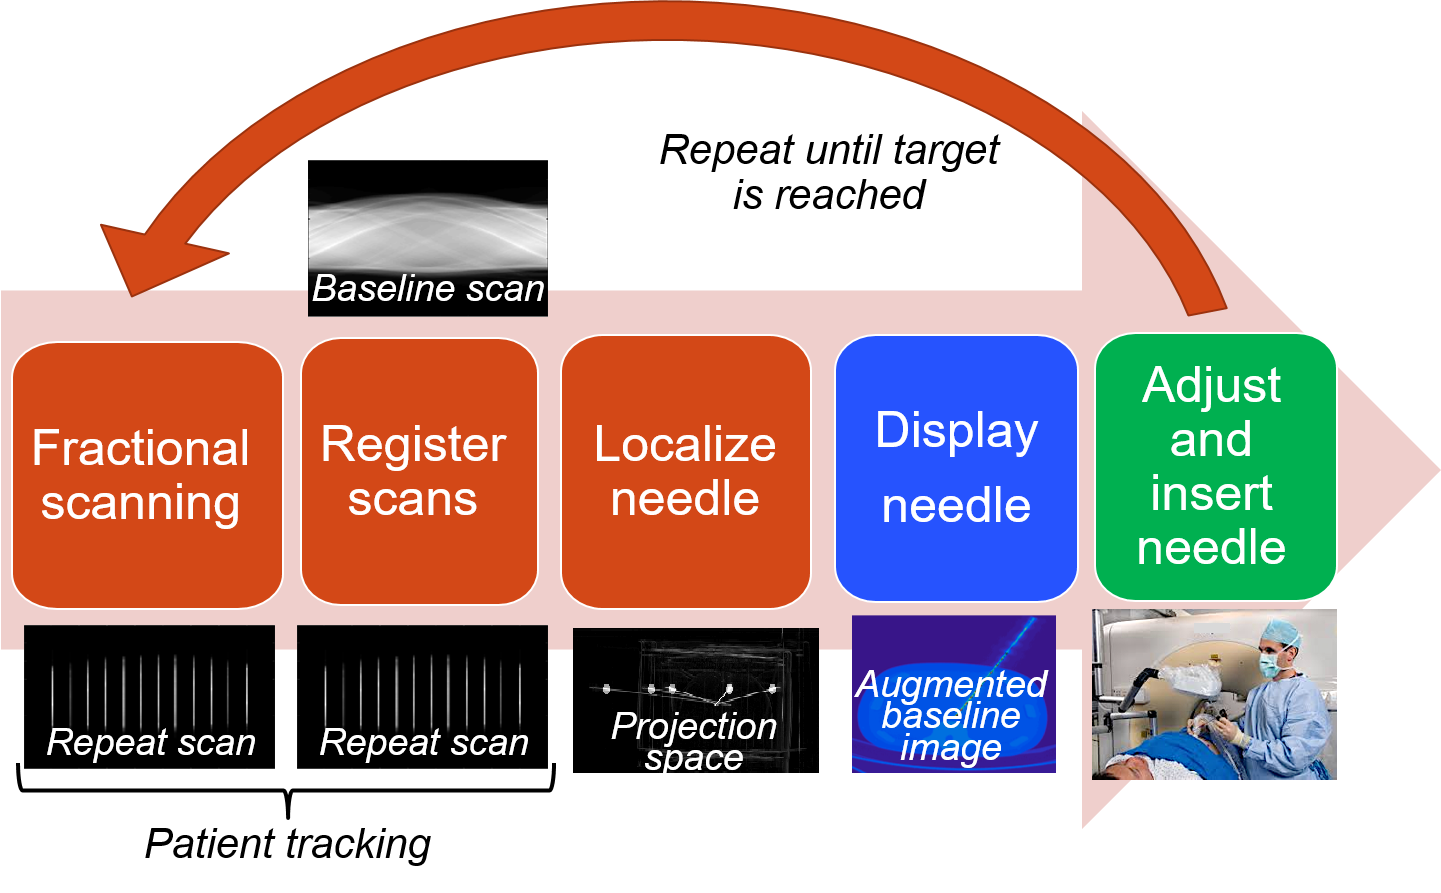
\includegraphics[width=15cm]{figures/needle+patient_tracking.png}
    \caption{\small{Illustration of image-less needle and patient tracking process in interventional radiology.}
}
    \label{fig:figures/needle+patient_tracking.png}
\end{figure*}

\section{Future Work}

The methods described in this thesis take advantage of sparse sampling in the view-angle domain during the CT acquisition process. However, to achieve the potential of substantial dose reduction, the scanning protocol and hardware itself must be altered in ways that are beyond the scope of this thesis. For example, some variants of dual-energy CT scanners switch the tube voltage between higher voltage (140kV) to lower voltage (80kV) every 1$^\circ$ 
\cite{goo2017dual}. By alternatively switching the voltage between high and low and with a wider angular spacing of 10$^\circ$-20$^\circ$, an x-ray dose reduction of $\times$10-50 can be achieved.

A different application to the low-dose rigid registration algorithm presented in this thesis is investigated by Shamul et al. \cite{shamul2017radon}. The goal of this work is to combine the baseline scan data with fractional repeat scanning to reconstruct CT images of the patient such that they incorporate any changes in the anatomy that may have occurred since the baseline scan, while achieving an x-ray dose reduction compared to a full repeat scan. In this approach a map of changed regions is computed based on comparisons in Radon space (made possible thanks to Radon space rigid registration), and consequently sparse scanning is performed such that only rays passing through the changed regions are acquired, enabling the reduction of x-ray dose. Then, the repeat and baseline data is combined in Radon space so that an image reconstruction can be computed using well known reconstruction methods. It is noted that this approach extends the hardware requirements from a CT scanner to not only support fractional scanning of view angles, but also to dynamically adjust its collimator as the gantry rotates so that only beams of interest are scanned.

Further work yet to be published by Adelman et al. extends rigid registration in Radon space to simultaneous deformable registration and image reconstruction based on a similar scheme of sparse view angles scanning and algebraic image reconstruction. This work has the potential to bring the promise of dose reduced applications to clinical procedures in which deformations cannot be neglected.

We expect that our approach to x-ray dose reduction will have a significant impact on the ongoing effort to lower doses of ionizing radiation in radiology, as manufacturers adopt new technologies in CT scanners enabling the rise of novel algorithms promising the benefit of reduced radiation-related risk to patients.